\section{Model}
\label{sec:model}

The basic element of our model is a \tg, which represents a graph that
evolves continuously over time.  A \tg represents evolution of graph
topology, i.e., the presence or absence of its vertices and edges, and
of the values of vertex and edge attributes.  Our choice to represent
continuous graph evolution is in contrast to a less-general discrete
snapshot-based representation.  We will discuss this distinction
further in Section~\ref{sec:related}.

Following the SQL:2011
standard~\cite{DBLP:journals/sigmod/KulkarniM12}, we adopt the {\em
  closed-open} period model, where a time period (or time interval)
represents a continuous set of time instances, starting from and
including the start time, continuing to but excluding the end time.

\begin{definition}[Time period]
A {\em time period} \\$p = [start, end)$ is an interval of the
  continuous time domain $T$, subject to the constraint $start < end$.
\label{def:period} 
\end{definition}

\begin{figure}
\centering
%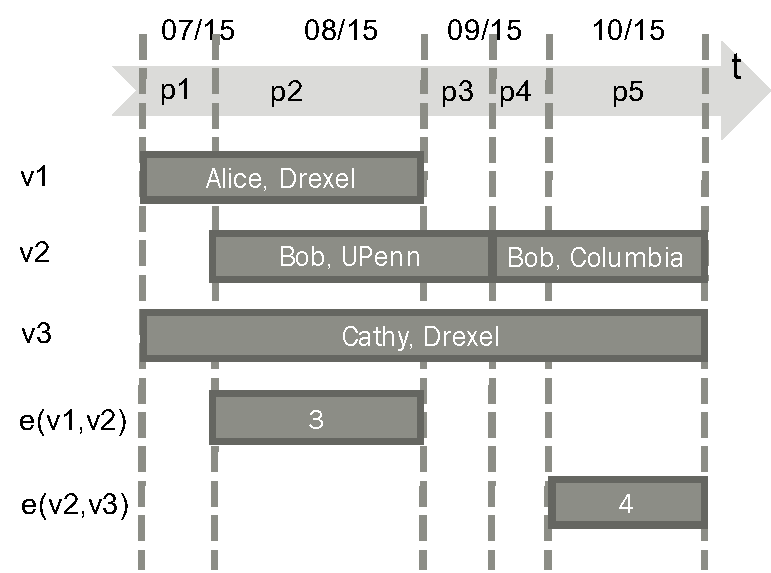
\includegraphics[width=2.5in]{figs/T1_relations.pdf}
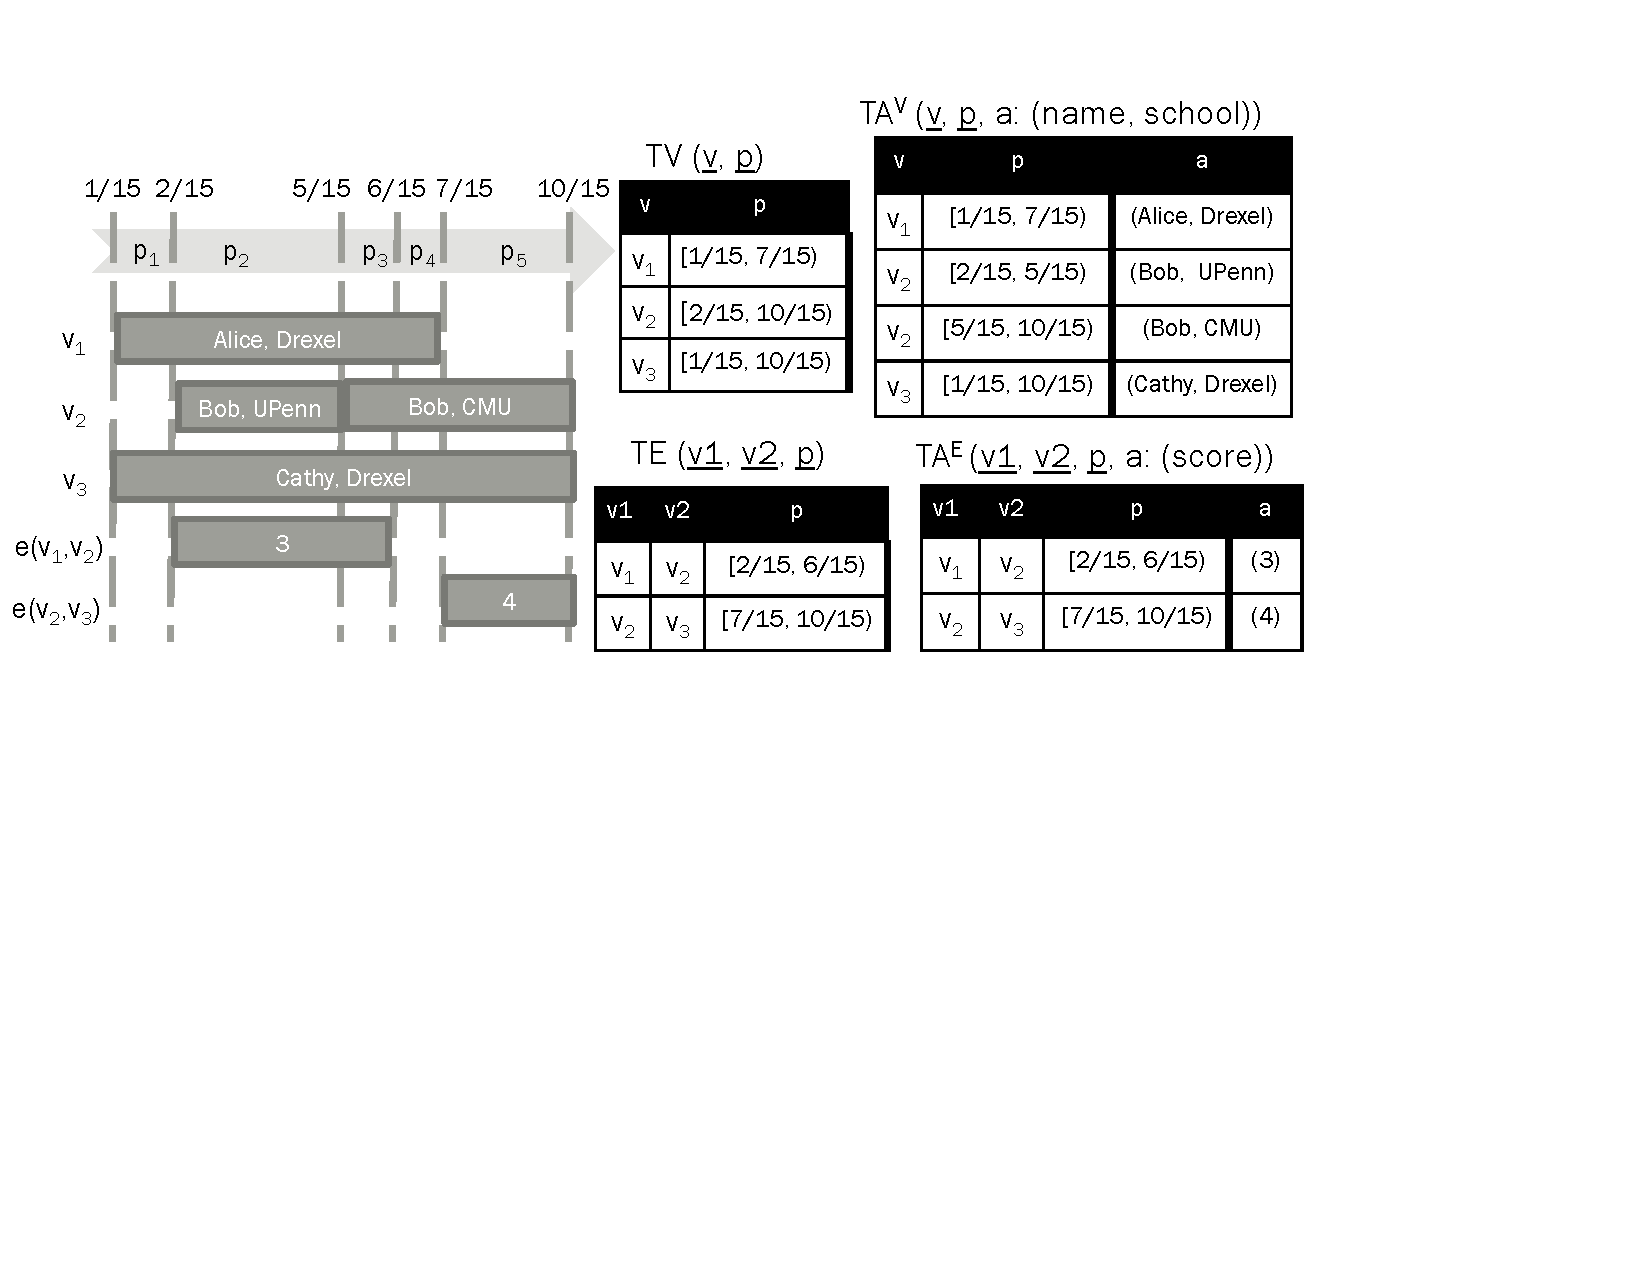
\includegraphics[width=3.5in]{figs/T1_rel_tab.pdf}
\caption{Vertex-edge representation of \tg \insql{T1}.}
\label{fig:tg_ve}
\end{figure}

\eat{\begin{figure}
\centering
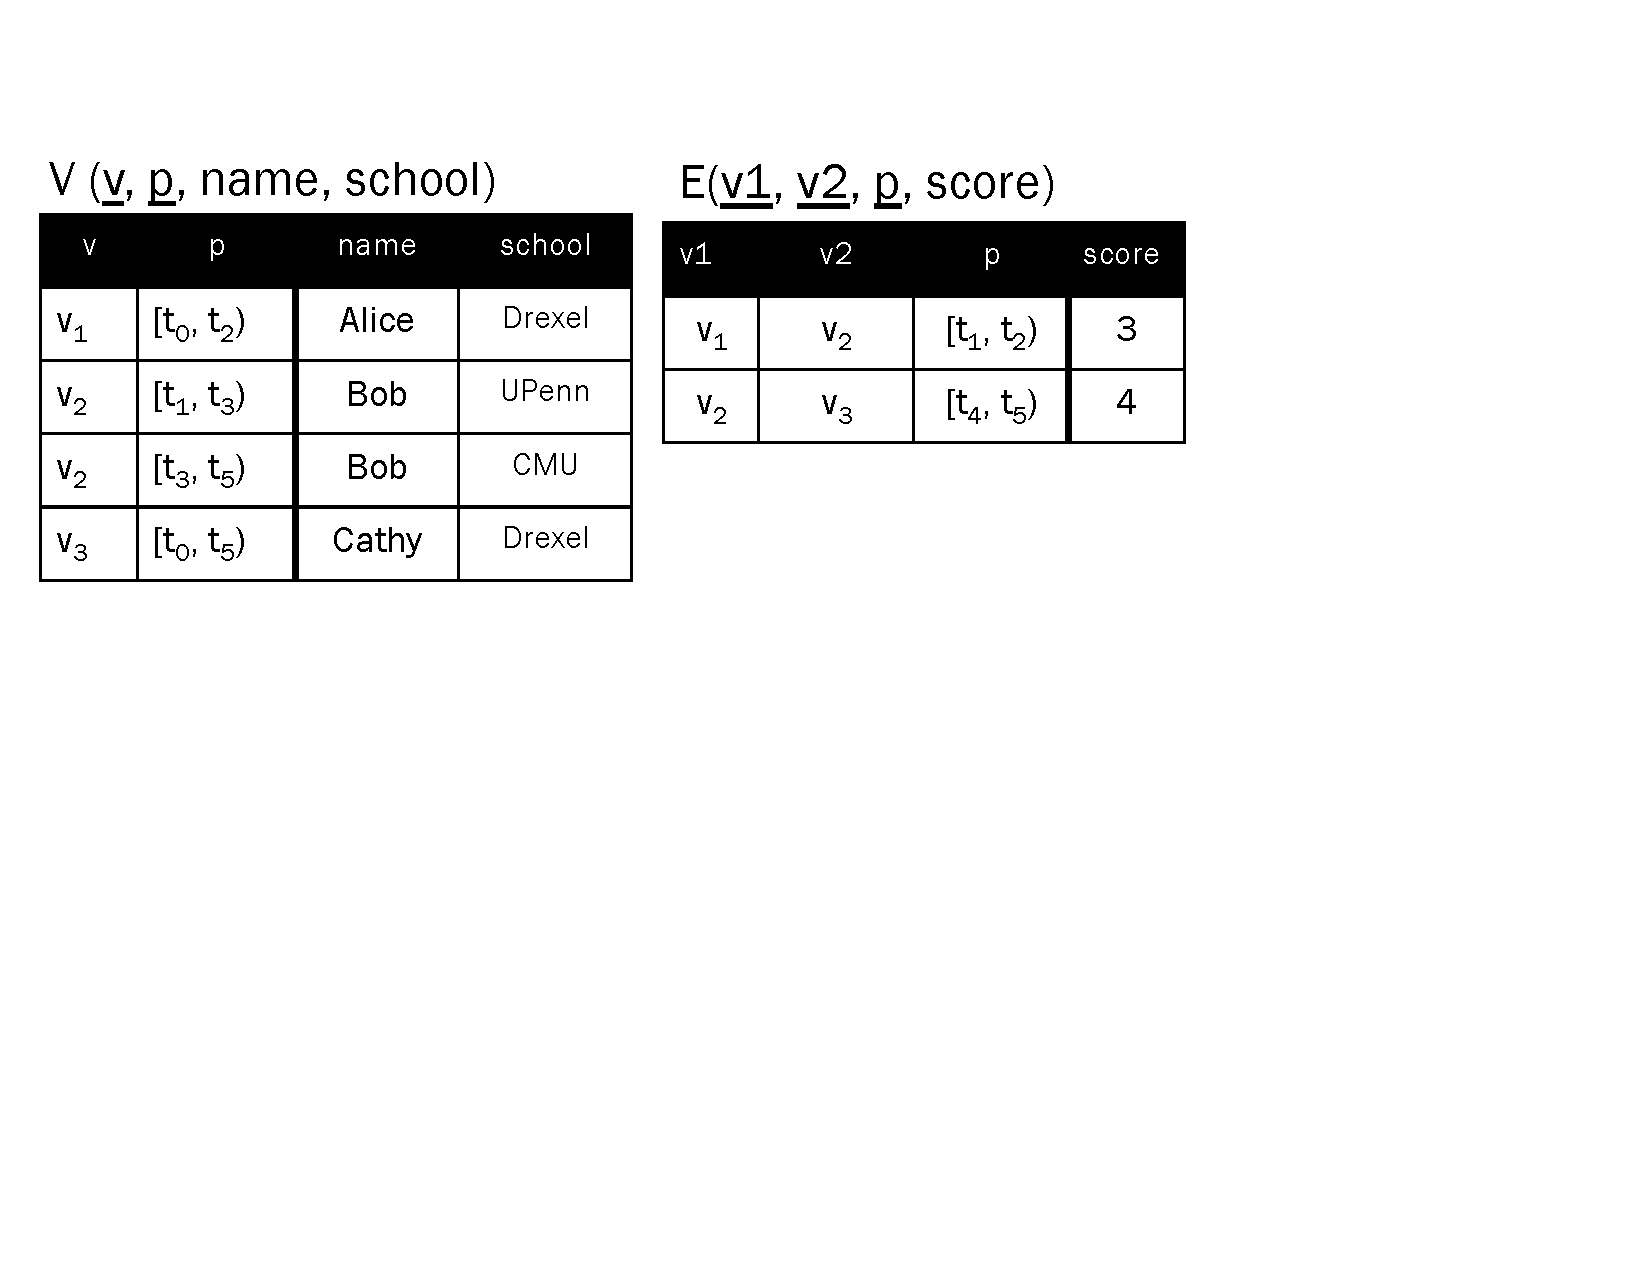
\includegraphics[width=3in]{figs/T1_tables.pdf}
\caption{\tg \insql{T1} as a pair of temporal SQL relations.}
\label{fig:tg_tab}
\end{figure}}

\begin{figure}
\centering
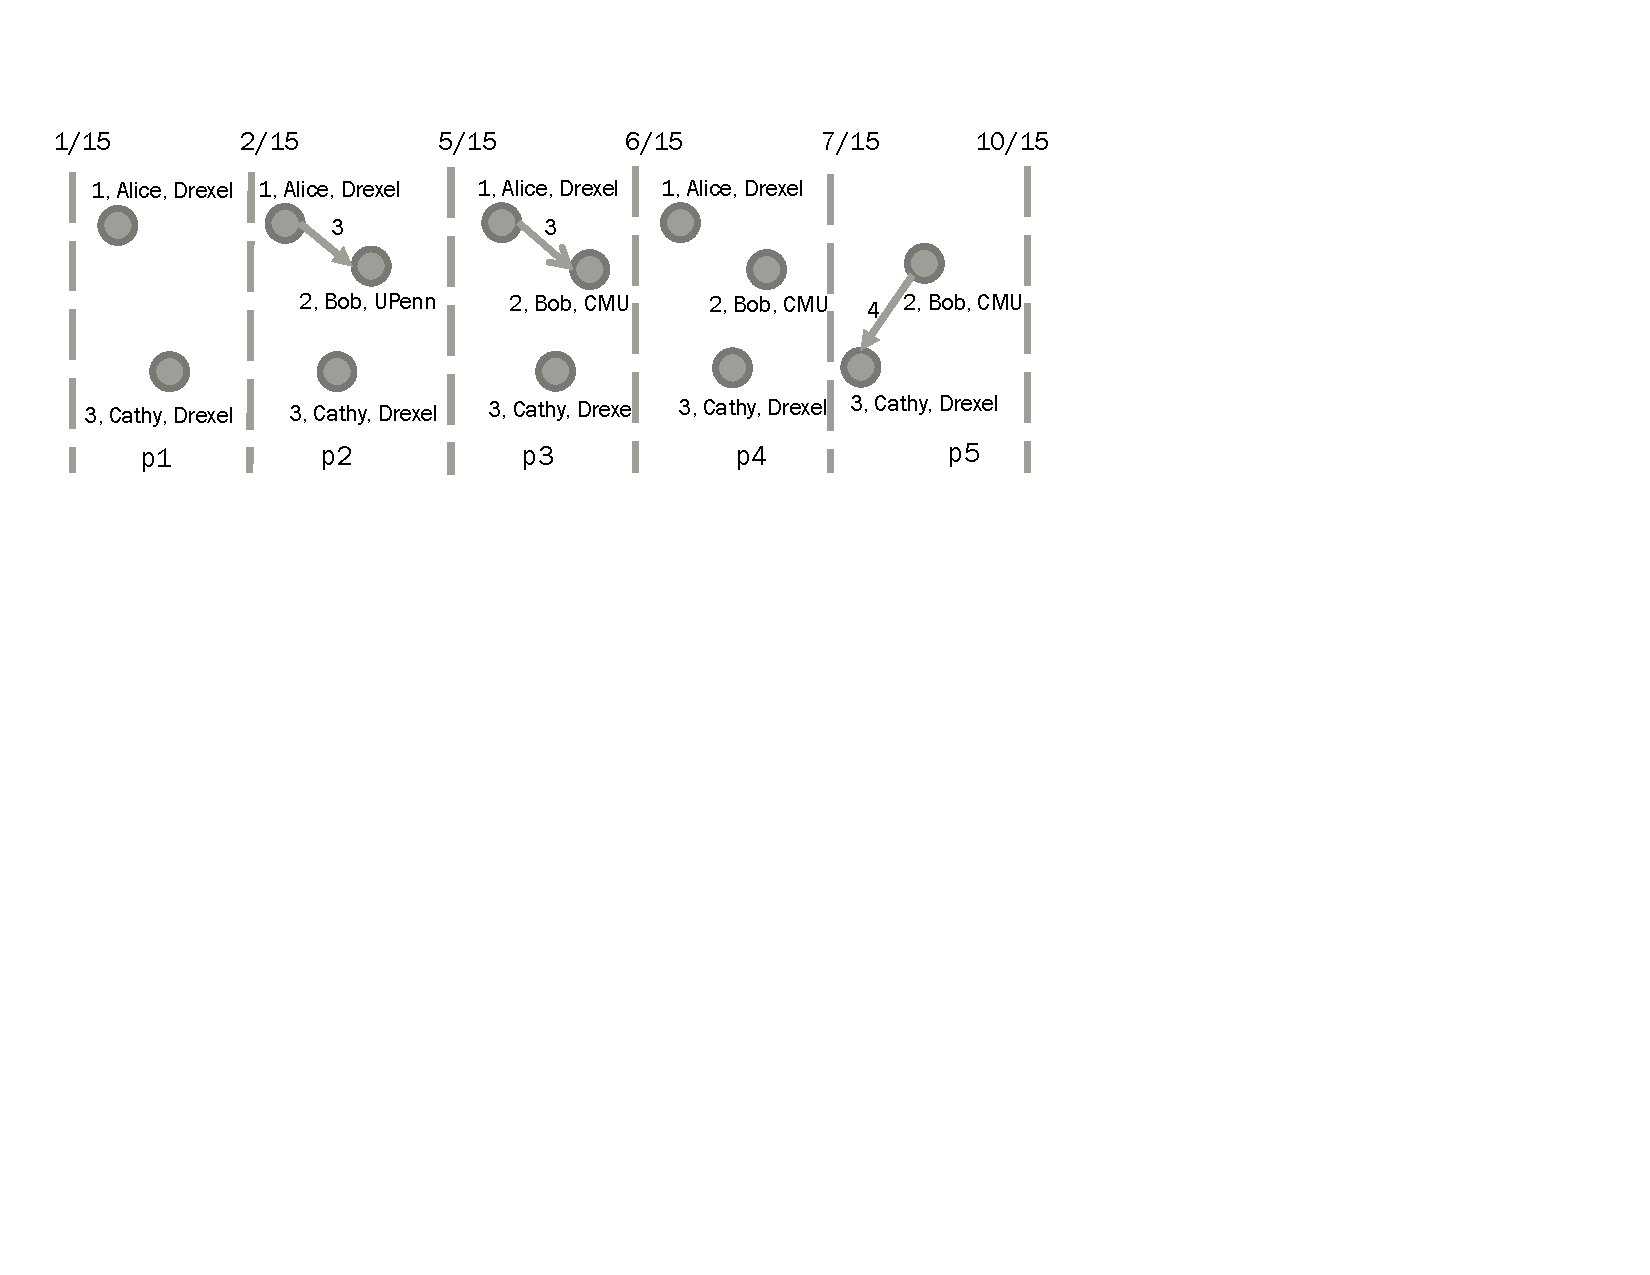
\includegraphics[width=3.5in]{figs/T1_graphs.pdf}
\caption{Representative graphs of \tg \insql{T1}.}
\label{fig:tg_rg}
\end{figure}

\eat{
It will be useful to quantify relationships between time periods $p$
and $q$ using the following Allen's relations~\cite{allen83}. }

\eat{\begin{itemize}
\item $p equal q$, defined as $p.start = q.start \wedge p.end = q.end$
\item $p overlaps q$, defined as $p.end > q.start$
\item $p meets q$, defined as $p.end = q.start$
\item $p during q$, defines as $p.start > q.start \wedge p.end < q.end$ 
\item $p starts q$, defined as $p.start = q.start \wedge p.end < q.end$
\item $p finishes q$, defined as $p.start > q.start \wedge p.end = q.end$
\end{itemize}}

We now define a \tg, the basic building block of our model that
represents an evolving graph with a pair of temporal SQL relations $V$
and $E$.  

\begin{definition}[TGraph]
An {\em evolving graph} \tg is a pair $(V; E)$, where $V$ is a finite
set of nodes with schema $V(\underline{v}, \underline{p}, a_1,
\ldots, a_n)$, and $E$ is a finite set of edges connecting pairs of
nodes from $V$, with schema $E(\underline{v_1}, \underline{v_2},
\underline{p}, b_1, \ldots, b_m)$, subject to the following
conditions:
\begin{multline}
\forall E(v_1, v_2, p)~~\exists V(v_1, p_1), V(v_2, p_2)~~| \\
                       \pred{p_1}{contains}{p}~\wedge~\pred{p_2}{contains}{p}
\label{def:tg:c1}
\end{multline}
\vspace{-0.5cm}
\begin{multline}
\forall V(v, p, a_1, \ldots, a_n)~~\nexists V(v, p', a_1, \ldots, a_n)~~| \\
                       \pred{p}{meets}{p'}~\lor~\pred{p}{contains}{p'}~\lor~\pred{p}{overlaps}{p'}
\label{def:tg:c2}
\end{multline}
\vspace{-0.5cm}
\begin{multline}
\forall E(v_1, v_2, p,  b_1, \ldots, b_m)~~\nexists E(v_1,v_2, p', b_1, \ldots, b_m)~~| \\
                       \pred{p}{meets}{p'}~\lor~\pred{p}{contains}{p'}~\lor~\pred{p}{overlaps}{p'}
\label{def:tg:c3}
\end{multline}
\vspace{-0.5cm}
\label{def:tg}
\end{definition}

The graph may be directed or undirected.  For undirected graphs we
choose a canonical representation of an edge, with $v_1 \leq v_2$
(self-loops are allowed).

Condition~\ref{def:tg:c1} in Definition~\ref{def:tg} states the
natural integrity constraint that an edge linking two vertices can
only exist during a time when both vertices exist.  Here,
$\pred{p}{contains}{q}$ is the Allen \predName{contains} relation with
equality~\cite{allen83}, defined as $p.start \leq q.start \wedge p.end
\geq q.end$.  Consider the vertex-edge representation of \tg
\insql{T1} in Figure~\ref{fig:tg_ve}, where edge $e(v_1,v_2)$ exists
during the entire period when both $v_1$ and $v_2$ exist, while edge
$e(v_2,v_3)$ exists only for a portion of the period when both $v_2$
and $v_3$ exist.

Conditions~\ref{def:tg:c2} and~\ref{def:tg:c3} in
Definition~\ref{def:tg} state that \tg is
coalesced~\cite{DBLP:conf/vldb/BohlenSS96}, which means that each
entity (vertex or edge) is represented exactly once for each time
period of maximal length when it is present, and when none of the
values of its attributes change.  Semantically, this means that the
entity exists continuously through the entire time period.  Here,
again, \predName{meets}, \predName{contains} and \predName{overlaps}
are the corresponding Allen relations~\cite{allen83}, with
equality. Consider the contents of $V$ and $E$ relations of \insql{T1}
in Figure~\ref{fig:tg_ve}, and note that there is a single tuple
corresponding to vertex $v_1$ in $V$, but two tuples corresponding to
$v_2$, because the value of the attribute $school$ of $v_2$ changed at
time $t_3$.

Coalescing requires that the system automatically merge adjacent and
overlapping time periods.  This operation, which is similar to
duplicate elimination in conventional databases, has been extensively
studied in the
literature~\cite{DBLP:conf/vldb/BohlenSS96,DBLP:journals/sigmod/Zimanyi06},
but is not fully supported by the SQL:2011 standard.

The \tg of Definition~\ref{def:tg}, although only partially enforcing
the constraints, can be implemented in temporal SQL as follows:

\begin{small}
\begin{verbatim}
CREATE TABLE V (
  v LONG,
  pstart DATE,
  pend DATE,
  PERIOD for p (pstart, pend),
  name varchar(32),
  school varchar(32),
  PRIMARY KEY (v, p WITHOUT OVERLAPS) )

CREATE TABLE E (
  v1 LONG,
  v2 LONG,
  pstart DATE,
  pend DATE,
  PERIOD for p (pstart, pend),
  score integer,
  PRIMARY KEY (v1, v2, p WITHOUT OVERLAPS),
  FOREIGN KEY (v1, PERIOD p) REFERENCES V(v, PERIOD p),
  FOREIGN KEY (v2, PERIOD p) REFERENCES V(v, PERIOD p) )
\end{verbatim}
\end{small}

The implementation above ensures that time periods corresponding to a
vertex (resp. edge) do not overlap, and that one does not contain the
other, but it does not prevent the existence of two adjacent time
periods, i.e., periods $p$ and $q$ for which $\pred{p}{meets}{q}$
holds.  That is, there may well be two tuples in $V$ for $v_1$, one
associated with $[t_0,t1)$ and the other with $[t_1,t_2)$ Another
    limitation of temporal SQL is that there is no convenient and
    efficient implementation of the coalesce operator (
    see~\cite{DBLP:reference/db/Bohlen09} for possible implementations).

Note that, while it is an important property of our logical model that
time periods be coalesced, eagerly coalescing is both expensive and,
in some cases, unnecessary.  We will discuss this in detail when
presenting \tg algebra (Section~\ref{sec:algebra}) and its
implementation (Section~\ref{sec:system}).

Non-key attributes of $V$ and $E$ are not restricted to be of atomic
types, but may, e.g., be maps or tuples.  Because of this, \ql
supports {\em schema evolution} in a \tg in much the same way as is
done in popular (non-temporal) graph databases like Neo4j.  At an
extreme, the vertex (resp. edge) relation will have a single
unstructured non-key attribute, which would store all attribute
information.  This representation has the usual advantages and
disadvantages --- flexibility of a schema-less representation at the
expense of missed performance optimization opportunities afforded by a
structured representation.

To conclude this section, let us revisit \tg \insql{T1} in
Figure~\ref{fig:tg_ve}.  Figure~\ref{fig:tg_rg} represents \insql{T1} as a
continuous sequence of graph states, each corresponding to a time
period during which no change occurred to the graph, in terms of
either topology or attribute values.

\eat{\begin{definition}[\rgs]
A {\em representative graphs} view of a \tg is a sequence of
(non-temporal) graphs associated with a sequence of consecutive
non-overlapping time periods.
\label{def:rgs} 
\end{definition}}

This view, to which we refer as \rgs of \insql{T1}, is computed from
properly coalesced $V$ and $E$ by (1) enumerating all time points
during which some change occured, i.e., that appear as either the
start or the end of some time period in $V$ and $E$, and (2)
generating pairs of adjacent time points. See Appendix for details.
\rgs is an important abstraction that will be useful to us in the next
section, where we present \tg algebra.

